\section{Zeeman Effect}\label{zeeman}
When no magnetic field is applied to a system, the magnetic dipoles of the orbital electron and spin have no preferred direction. 
The energy levels for all combinations of $L$ and $S$ (all $J$) are equivalent. 

% If a magnetic field is applied the magnetic moments interact
The application of a magnetic field causes an interaction between the spin-system magnetic moment and 
% with 
that field via the \index{Zeeman!Zeeman interaction}{Zeeman interaction}. 
The \index{Zeeman!Zeeman effect}{Zeeman effect} consists of atomic energy level splitting when an external magnetic field is imposed on a sample \cite{Nabokov2002}. 

Classically, we calculate the energy of a dipole in a magnetic field as
\begin{equation}
    E = -\vec{\mu}\cdot\vec{B}
    \label{eq:dipole_energy_scalar_prod}
\end{equation}
may be replaced with the Hamiltonian for a quantum mechanical system 
\begin{equation}
    \hat{H}_{\ce{Zeeman}} = - \hat{\vec{\mu}}\cdot \vec{B}. 
    \label{eq:}
\end{equation}

The negative sign is convention used to illustrate that the state of minimum energy is the state which the moment aligns to the magnetic field.

Thus distinct quantum systems with different $J$ and thus different projections of angular momentum ($m_J$). This difference in projected angular momentum accounts for the difference in energies between states with differing angular momentum.  

Considering $S=1/2$ system, which has twofold degeneracy, the Zeeman energy is the delta between the spin-system energy with the magnetic moment parallel and anti-parallel to the applied field. 


\begin{figure}[H]
    \begin{center}
        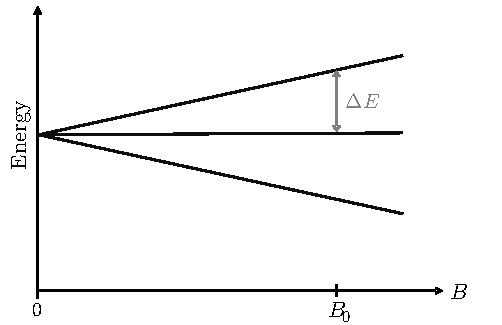
\includegraphics[width=0.6\textwidth]{figures/Zeeman.pdf}
        % \missingfigure{Figure showing the Zeeman energy for states separated by $m_s = \pm 1$}
    \end{center}
    \caption{Adapted from figure shown in the work by Gr\"{u}ne.}\label{fig:}
    \todo[inline, color=ediblue]{Write caption}
\end{figure}

The Hamiltonian to describe the energy is, using the total angular momentum form of \eqref{eq:orbital_magnetic_moment_operator_bohr_magneton_g_factor}, 
\begin{equation}
    \hat{H}_{\ce{Zeeman}} = g \mu_B \hat{\vec{S}}\cdot\vec{B}. 
    \label{eq:Zeeman_Hamiltonian}
\end{equation}

We simplify by aligning the field along the $z$ axis and reduce the scalar product to only the $z$ component. Now for a $S=1/2$ system i.e. $m_S = \pm 1/2$ we find the Zeeman energy by solving the Shr\"odinger equation 
\begin{equation}
    \hat{H}_{\ce{Zeeman}} \ket{S, m_S} = E_{\ce{Zeeman}}\ket{S, m_S} 
    % \label{eq:}
\end{equation}
which, to a factor is equivalent to, by \eqref{eq:zthcomponent}, to
\begin{equation}
    \hat{S}_{z} \ket{S, m_S} = m_S\ket{S, m_S}.
    % \label{eq:}
\end{equation}

Thus we find the two eigenvalues to be
\begin{equation}
E_+ =\frac{1}{2}g\mu_BB, \qquad E_-=-\frac{1}{2}g\mu_BB
    \label{eq:zeeman_energy}
\end{equation}
and thus the Zeeman energy is given by $g\mu_B B$. 



The $S=1/2$ system is thus doubly \index{degeneracy!degenerate}{degenerate} and the \index{degeneracy}{degeneracy} is lifted by the application a magnetic field. 
%
% These arguments may be generalised to a more complex system by considering the total angular momentum $J$ where the energy difference between states is given by 
% \begin{equation}
%    \Delta E = g_J \mu_B B. 
%     \label{eq:zeeman_energy}
% \end{equation}





